% Project 2 (Pump flow control) - bản standalone
\documentclass[12pt,a4paper]{report}

\usepackage[utf8]{inputenc}
\usepackage[T5]{fontenc}
\usepackage{mathptmx}
\usepackage{amsmath}
\usepackage{graphicx}
\usepackage{float}
\usepackage{tikz}
\usetikzlibrary{calc,positioning}

\graphicspath{{docs/}{docs/figures/}{figures/}}

\begin{document}

% ====== TITLE PAGE ======
\begin{titlepage}
\centering
\vspace*{2cm}

{\Large \textbf{SPEC DỰ ÁN 2}\par}
\vspace{0.5cm}
{\LARGE \textbf{Điều khiển bơm tuyến tính và phản hồi dòng}\par}

\vspace{1.5cm}
{\large Tài liệu đặc tả kỹ thuật (Standalone)\par}

\vfill
{\large \today\par}
\end{titlepage}

\tableofcontents
\clearpage

% ====== MAIN CONTENT ======
\chapter{Dự án 2 --- Điều khiển bơm tuyến tính và phản hồi dòng (Flow Control)}

\section{Mục tiêu và phạm vi}
Mục tiêu của khối là điều chỉnh công suất bơm DC 12V linh hoạt và ổn định theo tải thông qua phản hồi \textbf{dòng điện motor}. Hệ thống hỗ trợ hai chế độ:
\begin{itemize}
  \item \textbf{Manual mode}: đặt PWM theo biến trở/slider HMI.
  \item \textbf{Auto mode}: tự điều chỉnh PWM theo dòng đo được (giữ dòng mục tiêu hoặc giới hạn dòng).
\end{itemize}
Lưu ý: dòng điện là đại lượng phản hồi dễ đo; để ``giữ lưu lượng khí'' tuyệt đối cần bổ sung cảm biến lưu lượng.

\section{Sơ đồ khối (vòng kín)}

\begin{figure}[H]
\centering
\resizebox{\textwidth}{!}{%
\begin{tikzpicture}[
  node distance=10mm,
  block/.style={draw, rounded corners, align=center, minimum width=22mm, minimum height=10mm},
  arrow/.style={->, thick}
]
  \node[block] (set) {Setpoint\\(Manual PWM / $I_{set}$)};
  \node[block, right=10mm of set] (ctrl) {Controller\\(PI / step control)};
  \node[block, right=10mm of ctrl] (pwm) {PWM output\\ESP32};
  \node[block, right=10mm of pwm] (mos) {MOSFET\\Power stage};
  \node[block, right=10mm of mos] (mot) {Bơm DC 12V\\(motor)};
  \node[block, below=12mm of mos] (sen) {Cảm biến dòng\\ACS712 / Shunt+OpAmp};

  \draw[arrow] (set) -- (ctrl);
  \draw[arrow] (ctrl) -- node[above]{duty} (pwm);
  \draw[arrow] (pwm) -- (mos);
  \draw[arrow] (mos) -- node[above]{12V PWM} (mot);
  \draw[arrow] (sen) -- node[left]{ADC} (ctrl);
  \draw[arrow] (mot) |- (sen);
\end{tikzpicture}%
}
\caption{Sơ đồ khối vòng kín điều khiển bơm theo phản hồi dòng}
\label{fig:p2_block}
\end{figure}

\subsection{Yêu cầu I/O và giao tiếp}

\begin{table}[H]
\centering
\caption{Bảng I/O tối thiểu --- Dự án 2}
\begin{tabular}{|p{3.2cm}|p{2.2cm}|p{3.4cm}|p{6.2cm}|}
\hline
\textbf{Khối} & \textbf{Loại} & \textbf{Tín hiệu} & \textbf{Yêu cầu/ghi chú}\\
\hline
ESP32 $\rightarrow$ MOSFET & PWM output & GPIO\_PUMP\_PWM & 15--25 kHz (khuyến nghị), duty 0--100\%\\
\hline
ACS712/Shunt & Analog input & ADC\_I\_PUMP & Lọc RC hoặc lọc số; đo offset 0A khi bơm tắt\\
\hline
Diode flyback & Protection & --- & Nếu motor/bơm không có mạch dập xung\\
\hline
Nguồn 12V & Power & 12V\_IN & Chịu dòng bơm; tách nguồn logic 3.3V/5V từ buck\\
\hline
UART log & Debug & TX/RX & Log: duty, $I_{meas}$, mode, trạng thái lỗi\\
\hline
\end{tabular}
\end{table}

\begin{figure}[H]
\centering
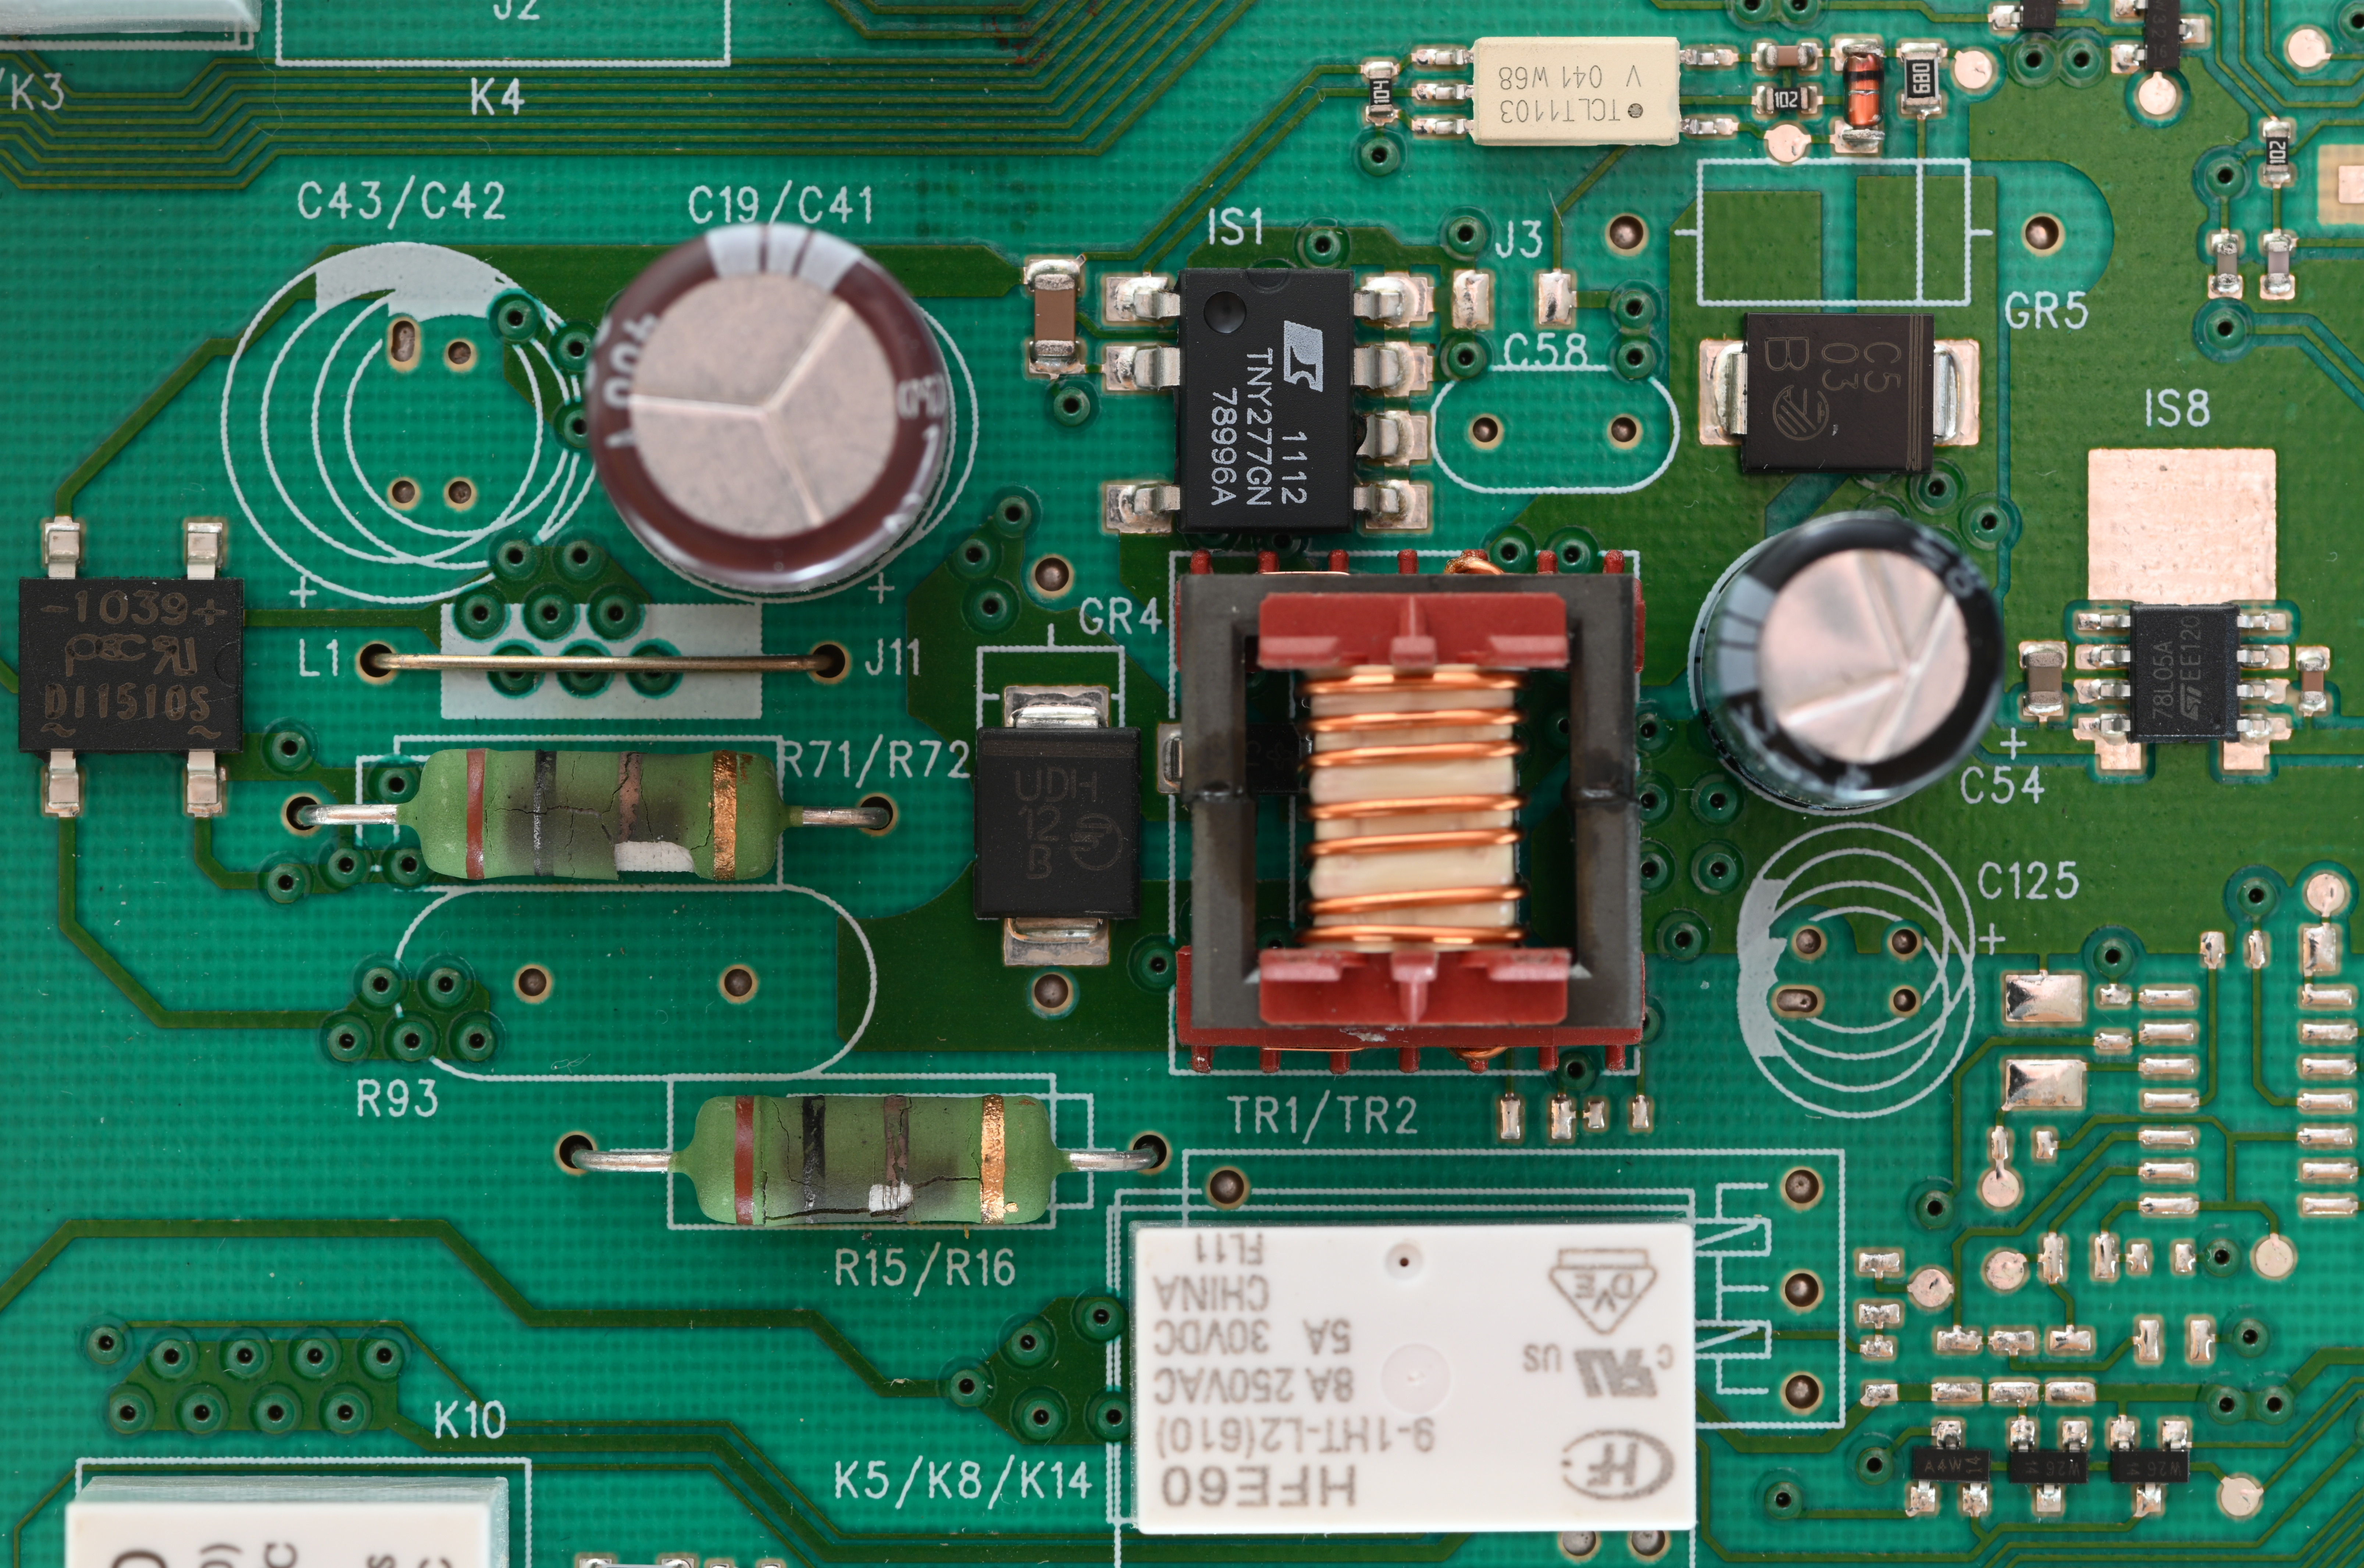
\includegraphics[width=0.7\textwidth]{figures/p2_power_stage_board.jpg}
\caption{Mạch công suất điều khiển tải với MOSFET và phần nguồn, minh hoạ cho khối công suất điều khiển bơm trong hệ thống.}
\label{fig:p2_power_stage_board}
\end{figure}

\section{Yêu cầu cơ khí và kích thước (bổ sung)}
\begin{itemize}
  \item \textbf{Bơm và đường ống}: xác định chuẩn đầu nối (phi 6/phi 8), chiều dài ống tối đa, và vị trí lắp van/nhánh T để giảm tổn thất áp.
  \item \textbf{Tản nhiệt MOSFET}: nếu bơm dòng lớn và PWM cao, cần heatsink hoặc module MOSFET có tản nhiệt sẵn.
  \item \textbf{Bố trí dây công suất}: dây motor đi xa cần tiết diện đủ và hạn chế chạy song song với dây ADC để giảm nhiễu.
\end{itemize}

\begin{figure}[H]
\centering
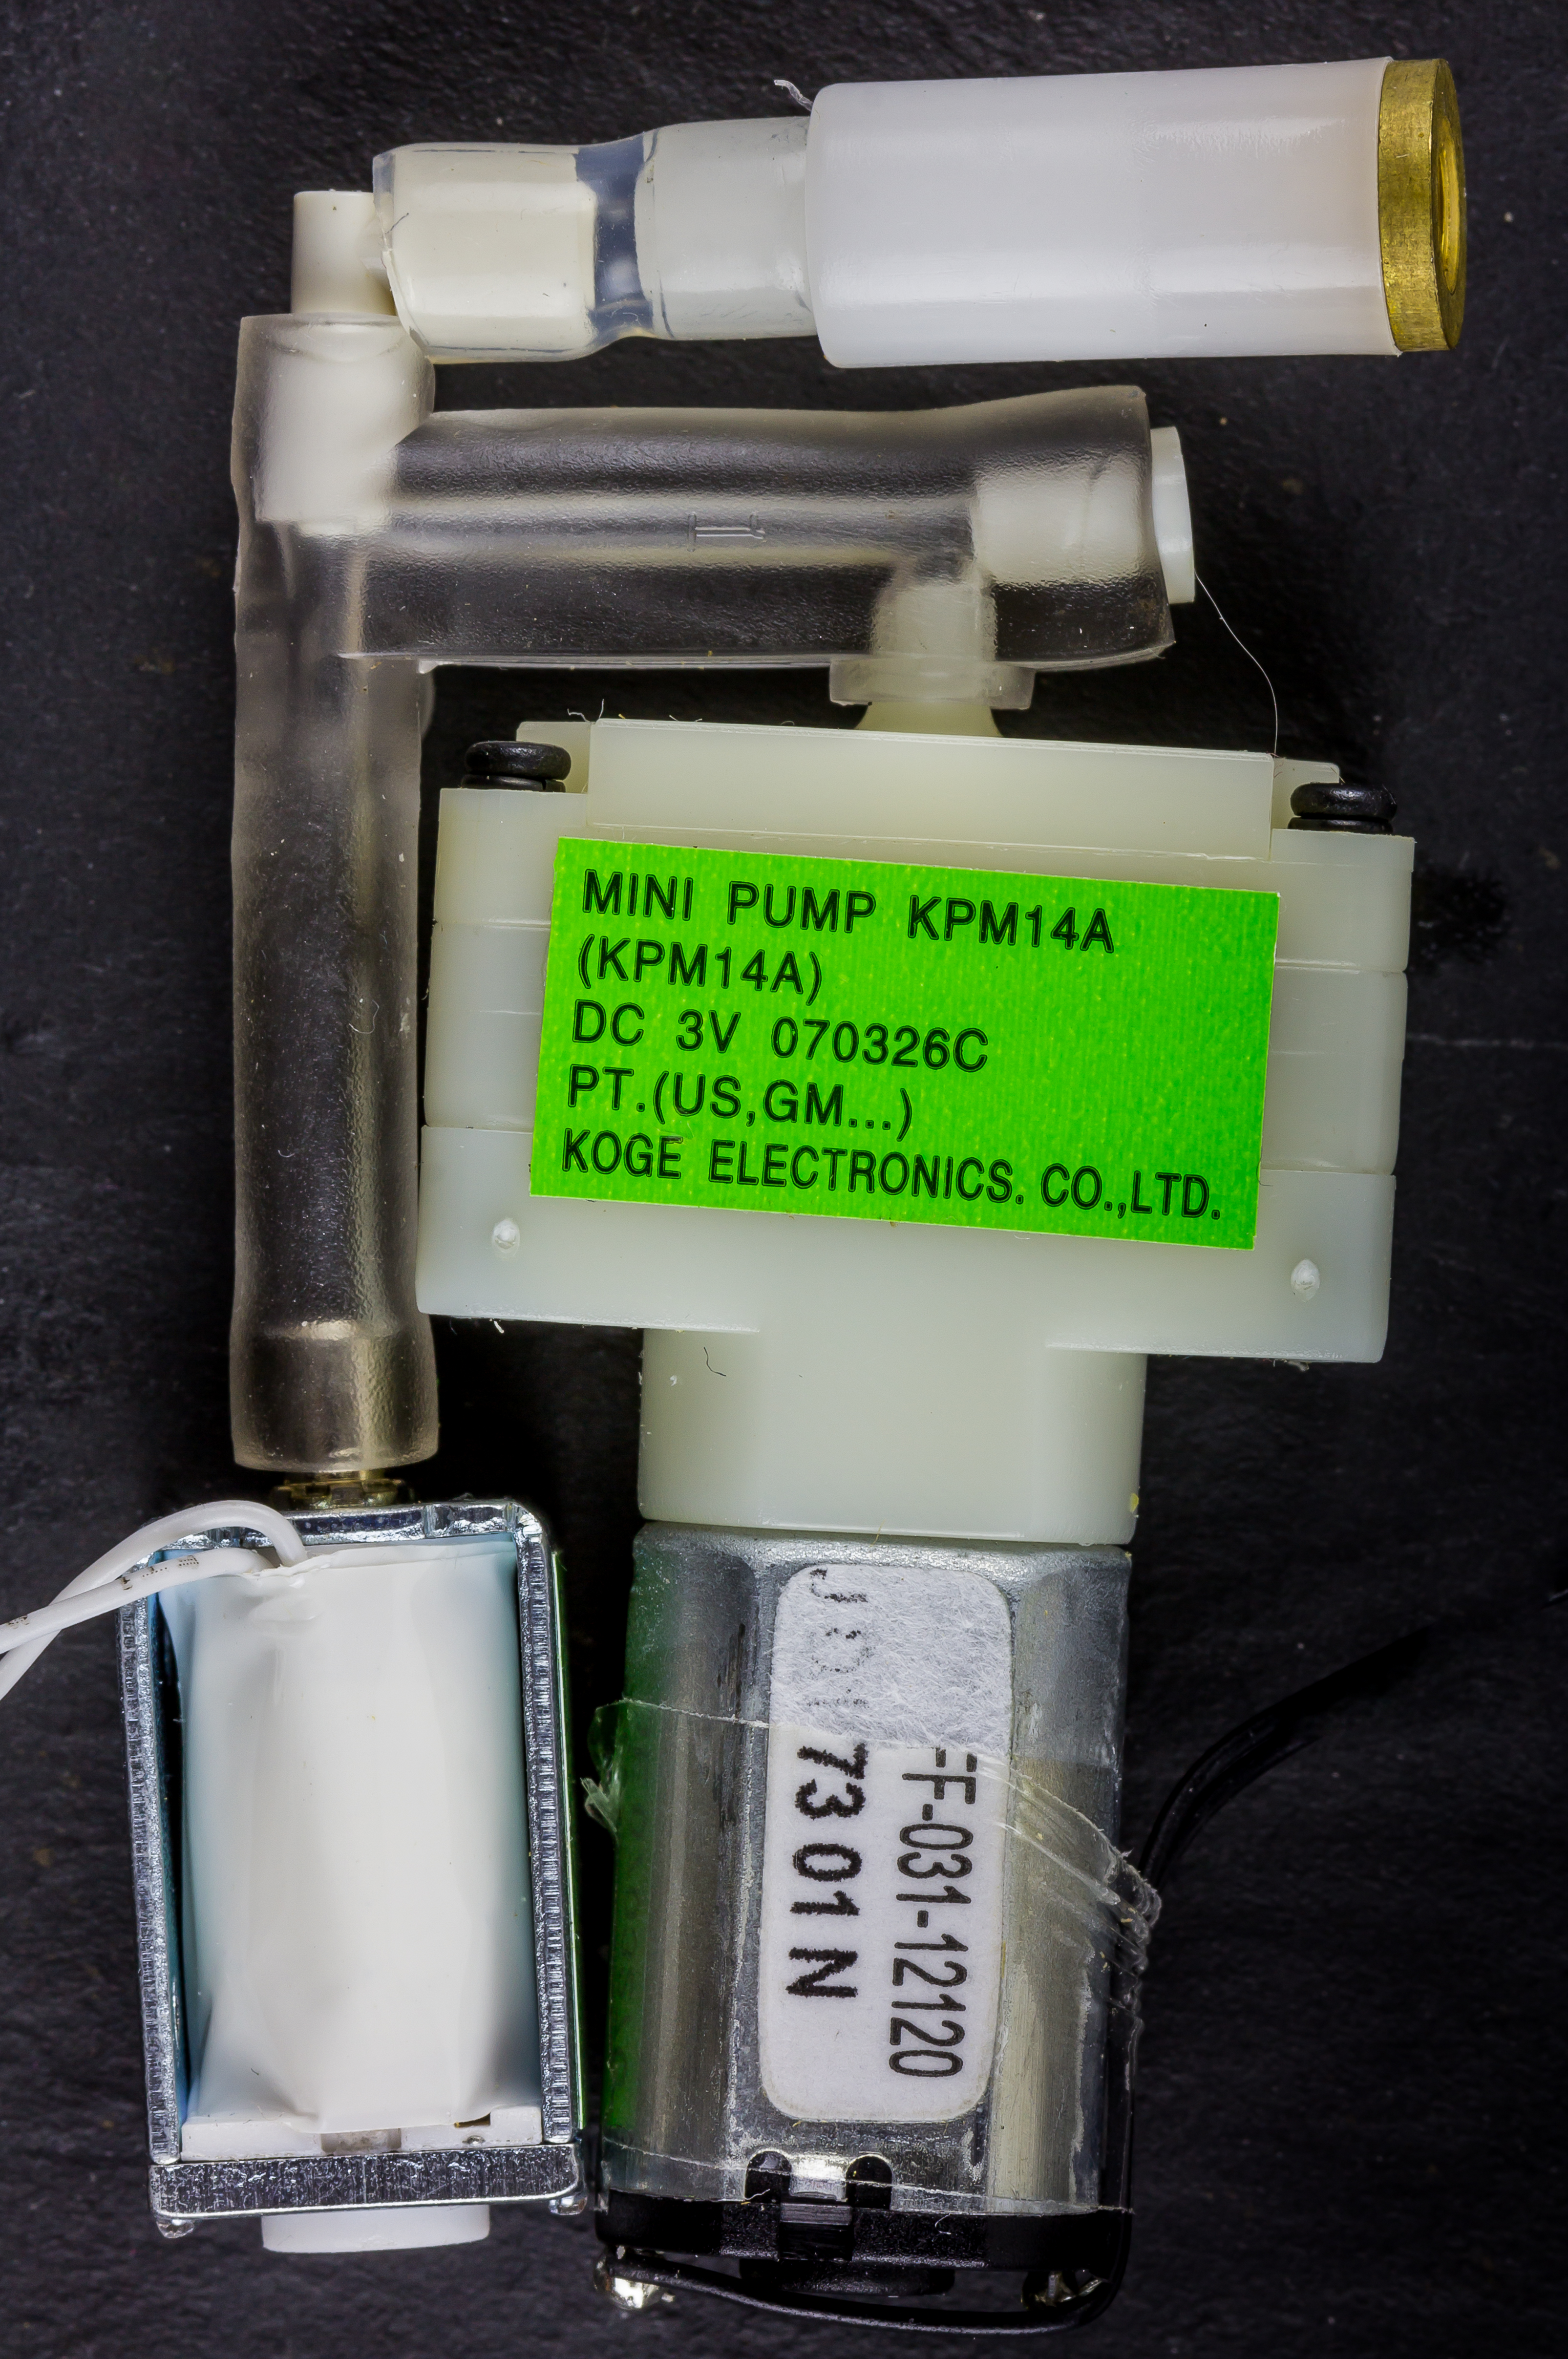
\includegraphics[width=0.45\textwidth]{figures/p2_dc_pump.jpg}
\caption{Bơm khí DC mini được sử dụng làm actuator; trong các bài test quá dòng, hệ thống điều chỉnh PWM hoặc dừng bơm để bảo vệ khi dòng vượt ngưỡng.}
\label{fig:p2_dc_pump}
\end{figure}

\subsection{Đặc tả đo dòng và hiệu chuẩn}
\begin{itemize}
  \item \textbf{PWM}: 15--25 kHz để giảm tiếng ồn; có thể giảm nếu phần cứng hạn chế.
  \item \textbf{ADC}: lấy mẫu 500 Hz--2 kHz kèm lọc số (EMA/moving average). Nếu cần độ chính xác cao có thể đồng bộ theo pha PWM.
  \item \textbf{Hiệu chuẩn}: đo offset 0A khi bơm tắt; hệ số scale theo datasheet ACS712 hoặc gain op-amp.
  \item \textbf{Giới hạn hợp lệ}: nếu ADC ngoài dải hợp lý $\rightarrow$ báo lỗi cảm biến, đưa hệ về trạng thái an toàn.
\end{itemize}

\begin{figure}[H]
\centering
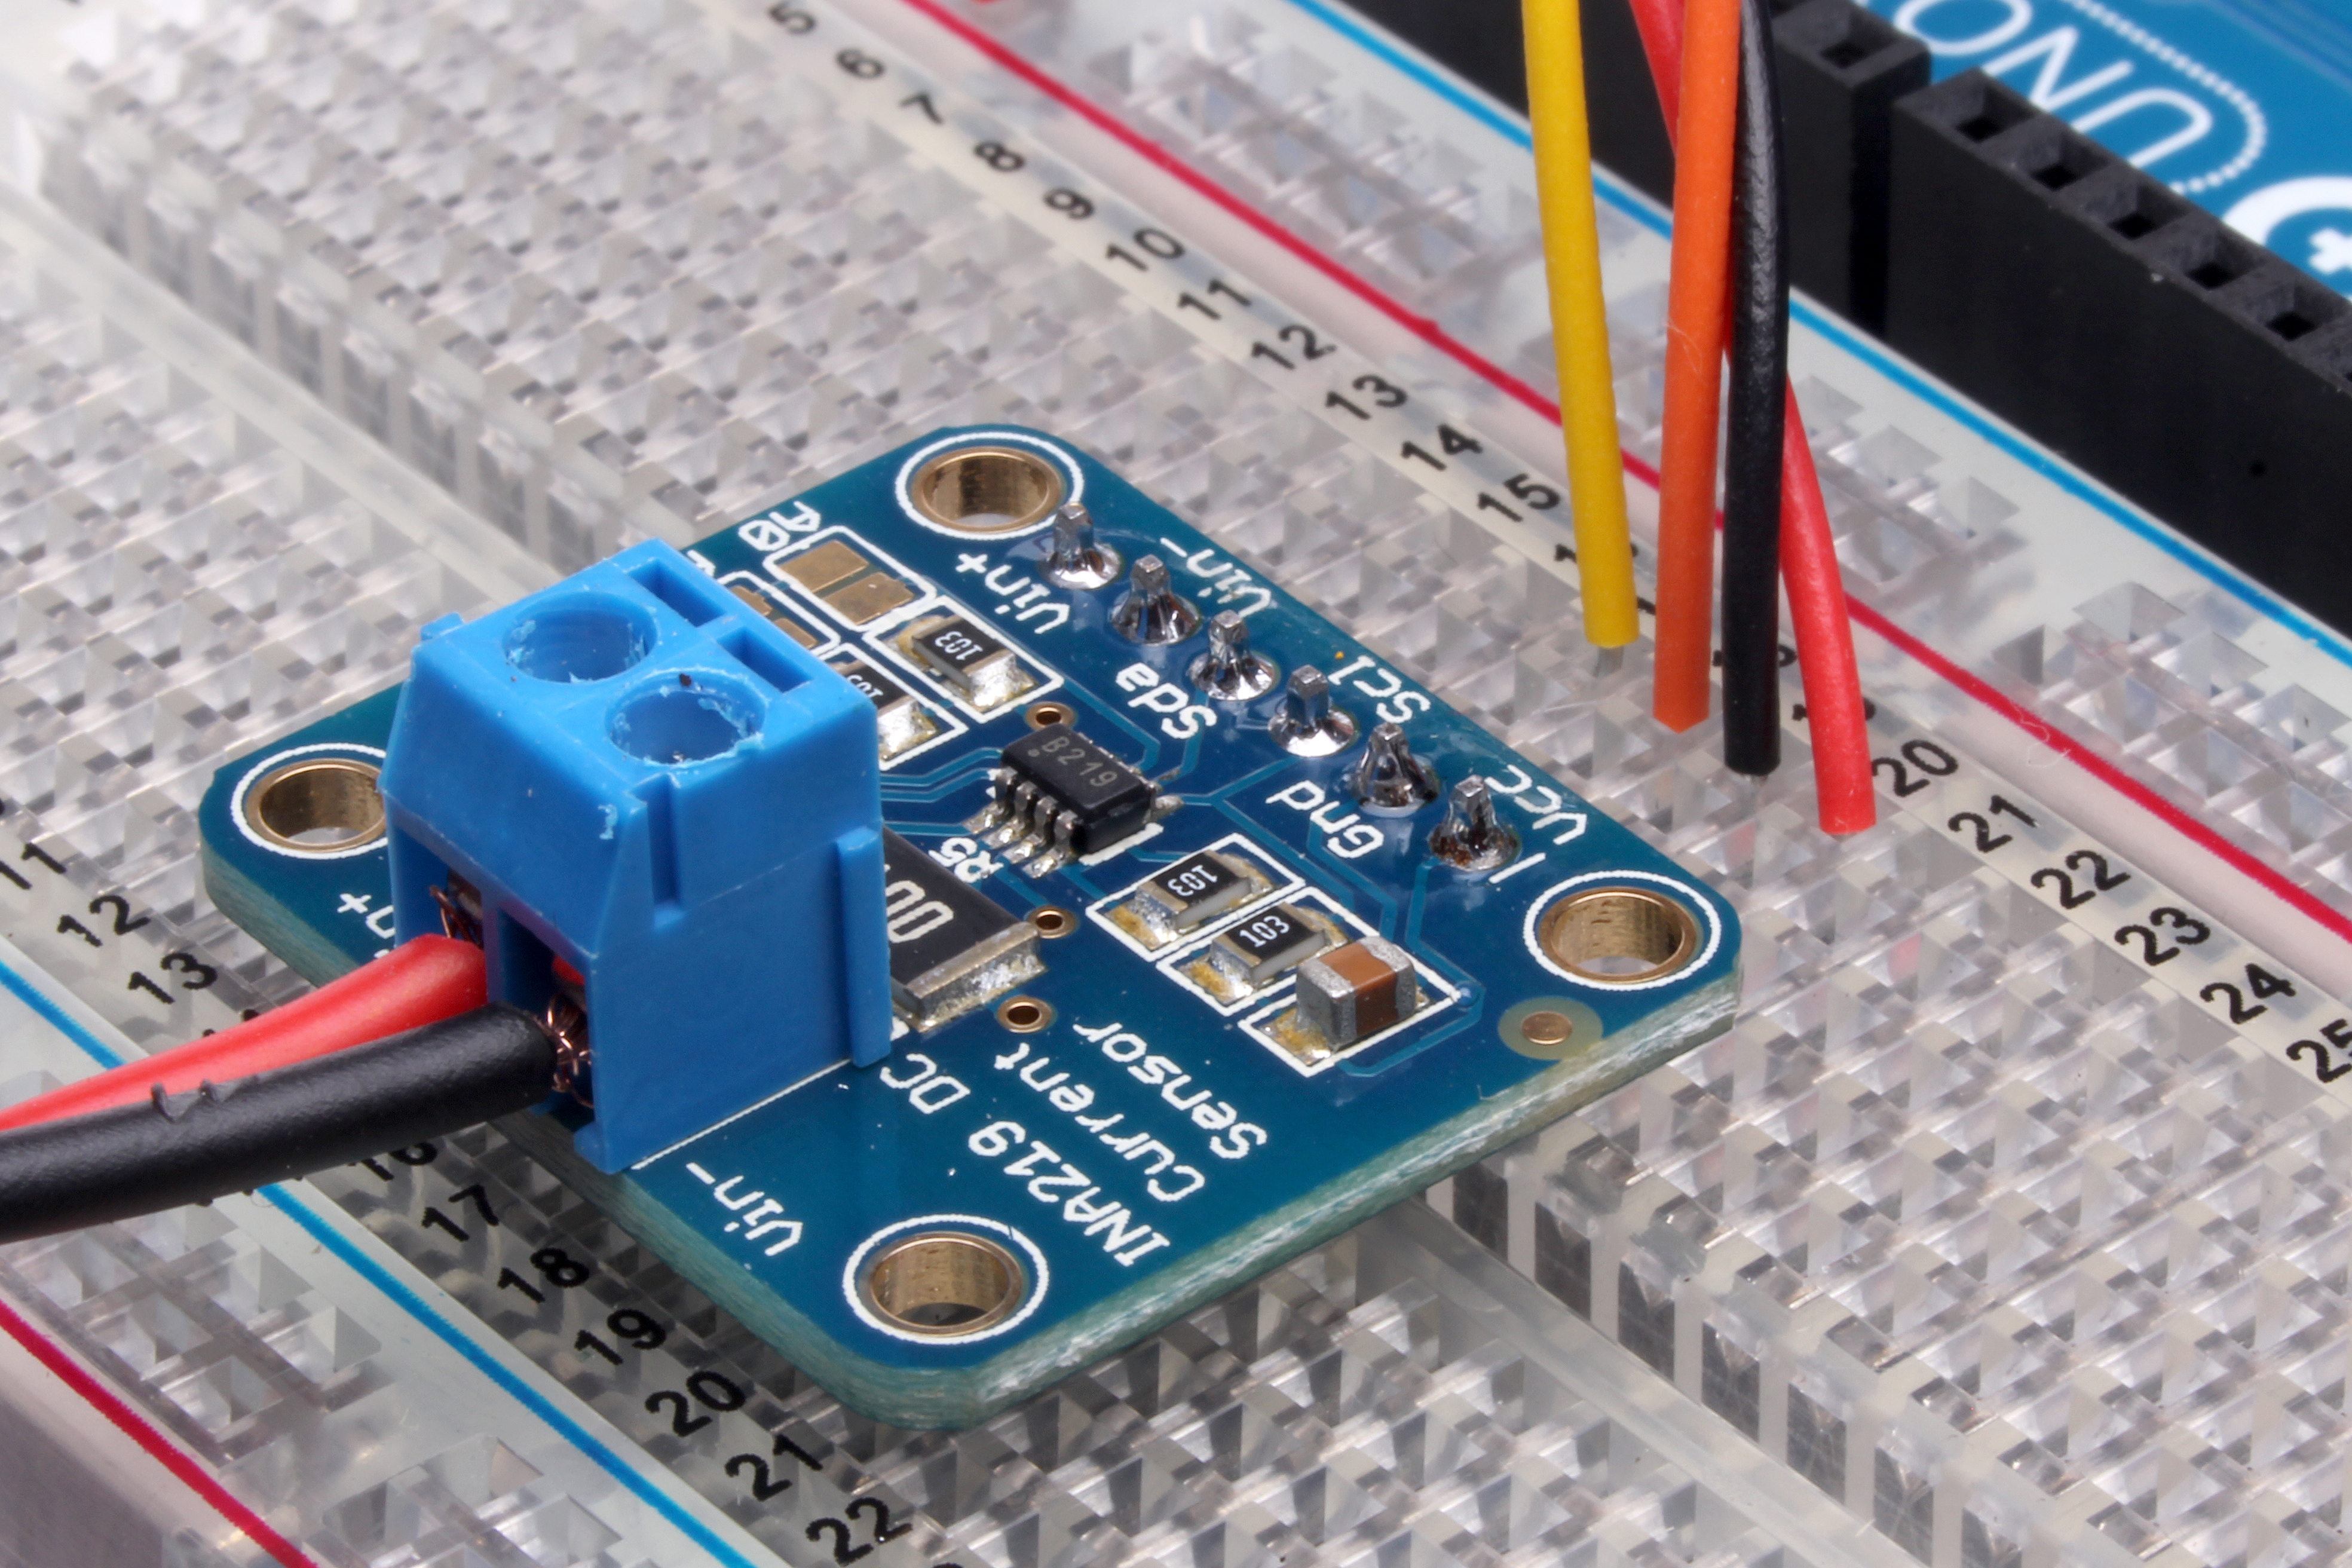
\includegraphics[width=0.7\textwidth]{figures/p2_current_sensor_module.jpg}
\caption{Module đo dòng một chiều dạng breakout (ví dụ INA219/ACS712) được lắp trên breadboard, minh hoạ khối cảm biến dòng trong vòng kín điều khiển bơm.}
\label{fig:p2_current_sensor_module}
\end{figure}

\section{Luật điều khiển (Auto mode --- đề xuất)}
Trong chế độ Auto, có thể lựa chọn một trong hai mục tiêu:
\begin{itemize}
  \item \textbf{Giữ dòng mục tiêu} $I_{set}$: $e = I_{set} - I_{meas}$, điều chỉnh duty theo PI hoặc tăng/giảm theo bước.
  \item \textbf{Giới hạn bảo vệ} $I_{max}$: nếu $I_{meas} > I_{max}$, giảm duty nhanh hoặc ngắt tạm và báo lỗi.
\end{itemize}

\section{Kiểm thử tối thiểu (acceptance)}
\textbf{Các bài test khuyến nghị}:
\begin{itemize}
  \item Manual: thay đổi slider $\rightarrow$ duty thay đổi tuyến tính, bơm đáp ứng.
  \item Auto: đặt $I_{set}$ $\rightarrow$ duty tự điều chỉnh để $I_{meas}$ hội tụ (không dao động mạnh).
  \item Overcurrent: cưỡng bức tải nặng $\rightarrow$ hệ thống giảm duty/ngắt và báo lỗi đúng.
\end{itemize}

\section{Kết nối với mạng WiFi mesh của hệ thống}
Node bơm của dự án 2 cũng là một node con trong mạng WiFi mesh ESP32 (dự án 3). Node này nhận lệnh đặt mode (MANUAL/AUTO), giá trị $I_{set}$, $I_{max}$ và trạng thái enable từ root node, sau đó điều khiển PWM bơm tương ứng; đồng thời gửi telemetry dòng, PWM và trạng thái lỗi về gateway để HMI và backend hiển thị, ghi log.

\end{document}
